\documentclass{minimal}
\usepackage{tikz}
\usetikzlibrary{arrows.meta, positioning}

\tikzset{
    % Define arrow tip and style
    >=Stealth,
    econbox/.style={
        rectangle,
        rounded corners,
        draw=blue!80!black, ultra thick,
        fill=white,
        text width=7em,
        minimum height=2.2em,
        font=\bfseries\color{blue!90!black},
        text centered
    },
    econarrow/.style={
        -{Stealth[scale=1.2]},
        line width=2pt,
        color=teal!80!black,
        shorten >=2pt,
        shorten <=2pt
    }
}

\begin{document}

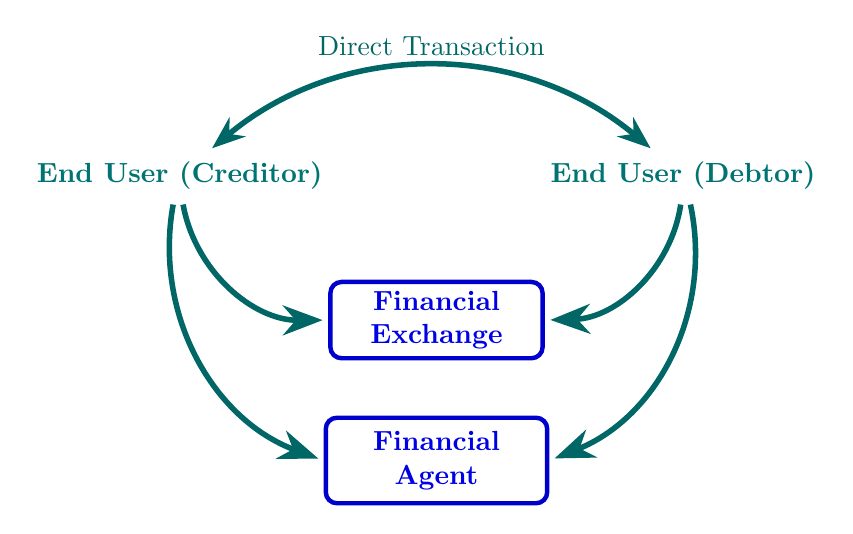
\begin{tikzpicture}[node distance=1.2cm, auto]

    % Nodes
    \node[econbox] (exchange) {Financial Exchange};
    \node[econbox, below=0.7cm of exchange, inner sep=5pt] (agent) {Financial Agent};
    % Dummy node for alignment
    \node[above=of exchange] (dummy) {};
    \node[right=of dummy, font=\bfseries\color{teal!90!black}] (debtor) {End User (Debtor)}
        edge[econarrow, bend left=40] (exchange.east)
        edge[econarrow, bend left=40] (agent.east);
    \node[left=of dummy, font=\bfseries\color{teal!90!black}] (creditor) {End User (Creditor)}
        edge[econarrow, bend right=40] (exchange.west)
        edge[econarrow, bend right=40] (agent.west)
        edge[econarrow,<->, bend left=40] node[font=\color{blue!70!black},anchor=south,above] {Direct Transaction} (debtor);

\end{tikzpicture}

\vspace{1em}
\emph{Adapted from a conceptual framework illustrating financial institutions in Economics.}

\end{document}